\section{Introducció}

\subsection{La fractal}
Una fractal és una figura, que pot ser espacial o plana, formada per components infinits. És a dir, si ens apropem veurem que no té fi. La seva principal característica és l'autosimilitud, exacta o no. Per exemple, en la figura \ref{fig:sierpinski}, podem veure el triangle de Sierpinski. Aquest té una autosimilitud exacta, doncs si ens apropem ens trobem amb la mateixa figura. En canvi, en la figura \ref{fig:mandelbrot}, el conjunt de Mandelbrot, no es autosimilar exacte, doncs si ens anem apropant ens surt la mateixa figura pero de vegades girada i això provoca que no sigui exacte.

\begin{figure}[h]
    \centering
    \begin{minipage}{.5\textwidth}
      \centering
      \includegraphics[width=.8\linewidth]{imatges/sierpinski.jpg}
      \captionof{figure}{Triangle de Sierpinski.}
      \label{fig:sierpinski}
    \end{minipage}%
    \begin{minipage}{.5\textwidth}
      \centering
      \includegraphics[width=.8\linewidth]{imatges/Captured_On_Mon_Dec__6_18-48-29_2021-.jpg}
      \captionof{figure}{Conjunt de Mandelbrot}
      \label{fig:mandelbrot}
    \end{minipage}
\end{figure}


\noindent Una característica que tenen tots els fractals és la seva dimensió. Aquesta moltes vegades es, fins i tot irracional. No sol ser 1 ni 2 ni 3. Per exemple, el triangle en la figura \ref{fig:sierpinski} és de dimensió $\frac{ln 3}{ln 2} \approx 1,585$. En canvi la dimensió del parímetre del conjunt de Mandelbrot, en la figura \ref{fig:mandelbrot} és de: 2. \n

\noindent Hi ha molts tipus de fractals, aquests son utilitzats desde els camps de l'art fins els camps de computació amb la compressió d'imatges i nombres pseudoaleatoris fins a la neurociència. També s'utilitzen per estudiar la formació de les estrelles, doncs els núbols de partícules es formen a partir del principi d'autosimilitud. Es pot estudiar fins i tot l'evolució del canvi climàtic. Doncs les fractals, en alguns casos, son sistemes caòtics.


\subsection{Nombres complexos}
Dins dels nombres existeixen per ordre: els nombres naturals ($\mathbb{N}$), els quals es troben dins dels enters ($\mathbb{Z}$), els quals formen part dels nombres racionals ($\mathbb{Q}$) i aquests, juntaments amb els irracionals formen part dels nombres reals ($\mathbb{R}$). Aquests amb els nombres imaginaris ($\mathbb{I}$) formen part dels complexos, representats amb el símbol $\mathbb{C}$.\n
\centerline {
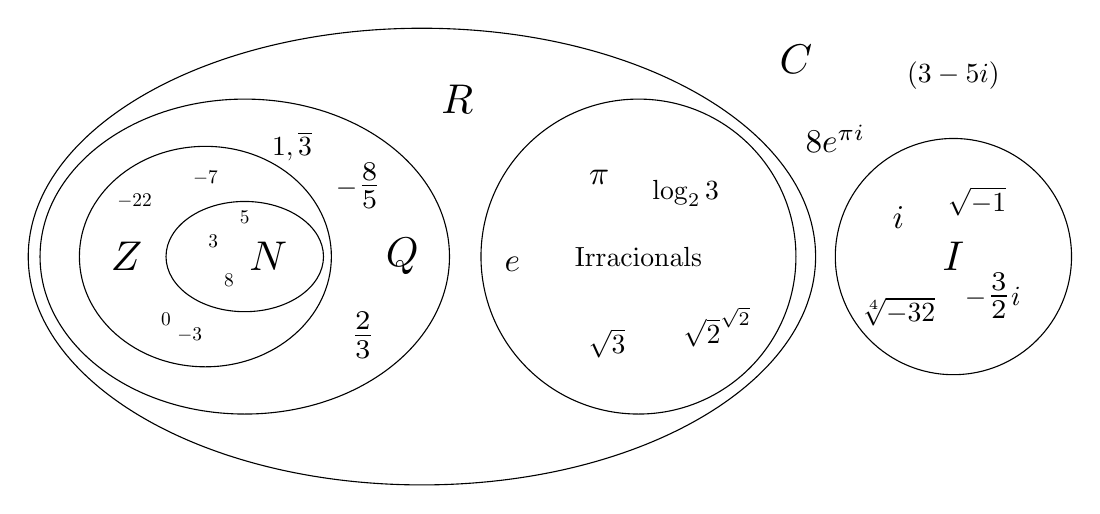
\begin{tikzpicture}
    %\draw[step=1cm,gray!15,very thin] (-5.9,-2.9) grid (8.9,2.9);

    % ELLIPSES:
    \draw (-1.5, 0) ellipse (1cm and 0.7cm);
    \draw (-2, 0) ellipse (1.6cm and 1.4cm);
    \draw (-1.5, 0) ellipse (2.6cm and 2cm);
    \draw (3.5, 0) ellipse (2cm and 2cm);
    \draw (.75, 0) ellipse (5cm and 2.9cm);
    \draw (7.5, 0) ellipse (1.5cm and 1.5cm);

    % LETERS:
    \draw (-1.2,0) node[anchor=center] {\scalebox{1.5}{$\mathbb{N}$}};
    \draw (-3,0) node[anchor=center] {\scalebox{1.5}{$\mathbb{Z}$}};
    \draw (0.5,0) node[anchor=center] {\scalebox{1.5}{$\mathbb{Q}$}};
    \draw (3.5,0) node[anchor=center] {Irracionals};
    \draw (1.2,2) node[anchor=center] {\scalebox{1.5}{$\mathbb{R}$}};
    \draw (7.5,0) node[anchor=center] {\scalebox{1.5}{$\mathbb{I}$}};
    \draw (5.5, 2.5) node[anchor=center] {\scalebox{1.5}{$\mathbb{C}$}};

    % NUMBERS:
    \draw (-1.9,0.2) node[anchor=center] {\scalebox{.7}{$3$}};
    \draw (-1.7,-0.3) node[anchor=center] {\scalebox{.7}{$8$}};
    \draw (-1.5,0.5) node[anchor=center] {\scalebox{.7}{$5$}};

    \draw (-2,1) node[anchor=center] {\scalebox{.7}{$-7$}};
    \draw (-2.5,-0.8) node[anchor=center] {\scalebox{.7}{$0$}};
    \draw (-2.9,.7) node[anchor=center] {\scalebox{.7}{$-22$}};
    \draw (-2.2,-1) node[anchor=center] {\scalebox{.7}{$-3$}};

    \draw (0,-1) node[anchor=center] {\scalebox{1.4}{$\frac{2}{3}$}};
    \draw (-.05,.9) node[anchor=center] {$-$\scalebox{1.4}{$\frac{8}{5}$}};
    \draw (-.9,1.4) node[anchor=center] {$1,\overline{3}$};

    \draw (3, 1) node[anchor=center] {\scalebox{1.2}{$\pi$}};
    \draw (3.1, -1.1) node[anchor=center] {$\sqrt{3}$};
    \draw (4.5, -.9) node[anchor=center] {\(\sqrt{2}^{\sqrt{2}}\)};
    \draw (1.9, -0.1) node[anchor=center] {\scalebox{1.2}{$e$}};
    \draw (4.1, 0.8) node[anchor=center] {$\log_2 3$};

    \draw (6.8, .5) node[anchor=center] {\scalebox{1.2}{$i$}};
    \draw (7.8, .7) node[anchor=center] {$\sqrt{-1}$};
    \draw (6.8, -.7) node[anchor=center] {$\sqrt[4]{-32}$};
    \draw (8, -.5) node[anchor=center] {$-$\scalebox{1.4}{$\frac{3}{2}$}$i$};

    \draw (6,1.5) node[anchor=center] {\scalebox{1.2}{\(8e^{\pi i}\)}};
    \draw (7.5,2.3) node[anchor=center] {$(3 - 5i)$};


    %\foreach \x in {-6,-5,-4,-3,-2,-1,0,1,2,3,4,5,6,7,8,9}
    %    \draw (\x cm,1pt) -- (\x cm,-1pt) node[anchor=north] {$\x$};
    %\foreach \y in {-3,-2,-1,1,2,3}
    %    \draw (1pt,\y cm) -- (-1pt,\y cm) node[anchor=east] {$\y$};

\end{tikzpicture}
}
Els nombres reals s'usen per mesurar quantitats reals, com ara longituds, velocitats, arees. I aquests nombres son suficients per a resoldre moltes equacions. Però existeixen algunes que simplement no es poden resoldre amb aquests numeros, com per exemple:
\[x^2 + 1 = 0 \; ; \; x = \pm\sqrt{-1}\]
No hi ha cap nombre que ens doni un resultat real per a \(\sqrt{-1}\). Sent aquest irreductible, li direm $i$, d'\textit{imaginary}.
\[\sqrt{-1} = i\]
Tenim, doncs, dues formes de representar els nombres complexos. La forma polar i la cartesiana, respectivament son: \newline \newline
\centerline{
\(
z = Me^{i\theta}
\left\{ \begin{array}{lcc}
        M \in \mathbb{R} \\
        \\ \theta \: en \: rad
         \end{array}
\right.\)
\(
\hspace*{6mm} ; \hspace*{6mm}
    z = a + bi
    \left\{ \begin{array}{lcc}
            a, b \in \mathbb{R}\\
            \\ bi \in \mathbb{I}
             \end{array}
   \right.
\)
}
%Aquesta forma ens indica l'angle directament en l'expressió i el seu módul. L'altra, en canvi, ens permet saver les seves "coordenades".
\subsubsection{El pla complex}
Si agafem la definició del nombre complex cartesià, tenim dues parts. La part real, $a$, i la part imaginaria, $bi$. D'aquesta manera podem mirar els nombres complexos com a punts o vectors, posant la part real en l'eix $x$ i en l'eix $y$ la part imaginaria. Per exemple:
\[z = 3 - 2i \; \rightarrow \; (3, -2)
\]
Així podem veure doncs que per a representar tots els nombres complexos podem utilitzar un pla. Si en aquest pla fem el que s'ha dit abans, l'$a$ en les $x$ i la $b$ en les $y$, hem creat el pla complex. \n
Representem uns quants nombres:
\[z_1 = 3 - 2i \; ; \; z_2 = 1 + 3i \; ; \; z_3 = -3 + 1i \; ; \; z_4 = 5e^{0,644i}\]
\newline
\centerline{
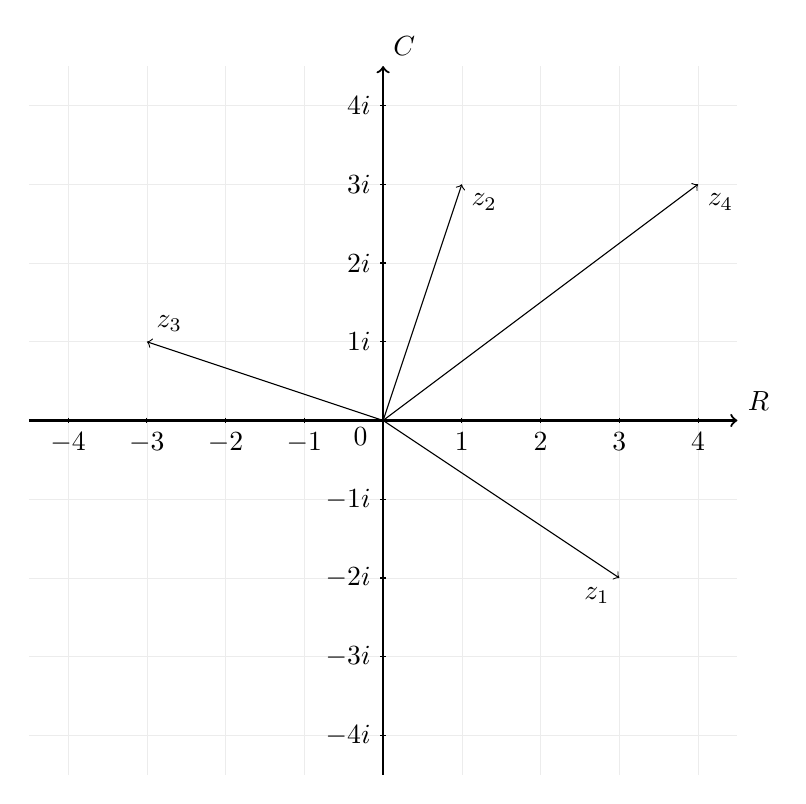
\begin{tikzpicture}
    \draw[step=1cm,gray!15,very thin] (-4.5,-4.5) grid (4.5,4.5);

    \draw[thick,->] (-4.5,0) -- (4.5,0) node[anchor=south west] {$\mathbb{R}$};
    \draw[thick,->] (0,-4.5) -- (0,4.5) node[anchor=south west] {$\mathbb{C}$};

    \draw (-0.5cm,1pt) node[anchor=north west] {$0$};

\foreach \x in {-4,-3,-2,-1,1,2,3,4}
    \draw (\x cm,1pt) -- (\x cm,-1pt) node[anchor=north] {$\x$};
\foreach \y in {-4,-3,-2,-1,1,2,3,4}
    \draw (1pt,\y cm) -- (-1pt,\y cm) node[anchor=east] {$\y i$};

    \draw[thin,->] (0,0) -- (3,-2) node[anchor=north east] {$z_1$};
    \draw[thin,->] (0,0) -- (1,3) node[anchor=north west] {$z_2$};
    \draw[thin,->] (0,0) -- (-3,1) node[anchor=south west] {$z_3$};
    \draw[thin,->] (0,0) -- (4,3) node[anchor=north west] {$z_4$};

\end{tikzpicture}
}

\subsection{Paral·lelització}
Quan programem, normalment el codi no és paral·lelitzat, doncs simplement li diem al processador que vagi fent línia a línia. Aquest mètode, quan tenim codi repetitiu, no és efficient. Seria millor si aquest codi repetitiu el poguessim executar multiples vegades a l'hora. Aquí és on entra la paral·lelització. \n
Aquesta la podem implementar de dues formes, per CPU o per GPU.
\subsubsection{CPU}
La CPU, \emph{Central Processing Unit}, és el component més important d'un ordinador. Seria com el cervell d'un animal. És que dona ordres a tothom. Aquesta compte amb diferents subprecessadors capaços de funcionar a l'hora i molt sovint es desaprofiten. \n
Estariem parlant d'uns pocs subporcessadors, en el meu cas en té 6. Però depen del processador, no hi ha un estàndar. \n
Per tant, seguint posant d'exemple el meu processador, podriem repetir la mateixa tasca 6 vegades a l'hora. Això ja ens dona molta aventatge. \n
Podriem estar temptants de dir que anirem 6 vegades més ràpid, però això no és així. L'acció d'enviar les dades per a realitzar el treball desitjat a un subprocessador consumeix temps, quan el subprocessador ha acabat ha de tornar les dades i s'han de sincronitzar tots els subprecessadors. Per tant, per a la realització de tasques petites no ens és eficient. \n
És útil quan volem realitzar tasques que consumeixin un temps gran.

\subsubsection{GPU}
La GPU, \emph{Graphics Processing Unit}, està enfocada en la idea de la paral·lelització. Aquesta unitat no es troba en tots els dispositius, ja que és prescindible, però molt útil. Originalment aquesta unitat va ser creada en la búsqueda de la rapidesa pel processament de cada píxel. Doncs és molt útil en videojocs i la generació de gràfics. \n
Últimament s'han trobat molt més usos d'aquesta unitat, com ara l'entrenament de \emph{Machine Learning} o la mineria de \emph{cryptomonedes} per exemple. \n
Al estar enfocada en aquesta idea de processar cada píxel, en el meu cas, té 1024 subprocessadors. Aquests son més petits que els de la CPU, per això hi han tants, però més eficients. \n
Aquest útlim ens serà útil en el càl·lcul de fractals.
